\documentclass{scrartcl}
\usepackage[english]{babel}
\usepackage{url}
\usepackage[utf8]{inputenc}
\usepackage{float}
%\usepackage[draft]{graphicx}
\usepackage{graphicx}
\usepackage{amsmath}
\usepackage{amssymb}
\usepackage{color}
\usepackage[table]{xcolor}
\usepackage{multirow}

\usepackage{amsfonts}
\usepackage{pgf}
%\usepackage{microtype}

\usepackage{todonotes}
\usepackage{subcaption}

\newcommand{\lmin}{\vec{l}_{\text{min}}}
\newcommand{\und}[2]{#1_{\vec{#2}}}
\newcommand{\imin}{\vec i_{\text{min}}}
\newcommand{\uc}{\und{u}{n}^{(c)}}

\newcommand{\abs}[1]{\left| #1 \right|}   %modulus
\newcommand{\avg}[1]{\langle #1 \rangle}  %average
\newcommand{\rf}{{\rm ref}}

\usepackage{verbatim}

\title{Applying the combination technique to linear initial value computations in GENE}
\subtitle{Version 0.2}
\author{Mario Heene}

\begin{document}

\maketitle

\section{Content}
We investigate the approximation quality and resource consumption when computing typical outputs of linear initial value computations in GENE with the sparse grid combination technique. The following outputs are investigated
\begin{itemize}
	\item the eigenvalue with the largest real part (\texttt{omega.dat})
	\item the corresponding eigenvector (\texttt{checkpoint})
	\item the moments of the particle distribution function and the particle, heat and momentum fluxes (\texttt{nrg.dat})
\end{itemize}

\section{Methodology}
\subsection{Sparse Grid Combination Technique}

The sparse grid combination technique computes the sparse grid approximation of a function $f$ by a weighted sum of partial solutions $f_{\vec{l}}$ on coarse and anisotropic Cartesian component grids $\Omega_{\vec l}$, scaled to the unit-hypercube. 
The discretization of each $d$-dimensional component grid $\Omega_{\vec l}$ is defined by the level vector $\vec l = (l_1,\cdots,l_d)^T$, 
which determines the uniform mesh width $2^{-l_i}$ in dimension $i$.
The number of grid points of a component grid is $|\Omega_{\vec l}| = \prod_{i=1}^d (2^{\vec{l}_i} \pm 1)$ 
($+1$ if the grid has boundary points in dimension $i$ and $-1$ if not).

In order to retrieve a sparse grid approximation $f_{\vec n}^{(c)} \approx f$ one can combine the partial solutions $f_{\vec{l}}(\vec{x})$ as 
\begin{equation}
	f_{\vec n}^{(c)}(\vec x) = \sum_{\vec l \in \mathcal I}c_{\vec l}f_{\vec l}(\vec x)\,,
	\label{eq:combination}
\end{equation}
where $c_{\vec l}$ are the combination coefficients and $\mathcal I$ is the set of level vectors used for the combination. $\vec n$ denotes the maximum discretization level in each dimension. It also defines the discretization of the corresponding full grid solution $f_{\vec n}$ on $\Omega_{\vec n}$.

There exist different approaches to determine the combination coefficients $\vec c_{\vec{l}}$ and the index set $\mathcal I$.
Here, we use
\begin{equation}
	f_{\vec n}^{(c)}(\vec x) = \sum_{q=0}^{d-1}(-1)^q
	\begin{pmatrix}
		d-1\\q
	\end{pmatrix}
	\sum_{\vec l \in \mathcal I_{\vec n,q}}f_{\vec l}(\vec x)
	\label{eq:combi}
\end{equation}
with the index set
\begin{equation}
	\mathcal I_{\vec n,q} = \{\vec l \in \mathbb N^d:|\vec l|_1= |\vec l_{\text{min}}|_1+c-q : \vec n \geq \vec l \geq \vec l_\text{min}\}\,,
	\label{eq:index_classic}
\end{equation}
where $\vec l_{\text{min}} = \vec n - c\cdot\mathbf{1}$, $c \in \mathbb N_0$ s.th. $\vec l_\text{min} \geq \mathbf{1}$ specifies a minimal resolution level in each direction, $\vec 1 = (1,\dots,1)^T$ and $\vec l \geq \vec j$ if $\vec l_i \geq \vec j_i~ \forall i$.

\subsection{Computation of eigenvalue $\lambda$}

The combined solution for $\lambda$ is computed according to Eq.~\eqref{eq:combi}
\begin{equation}
	\lambda^{(c)} = \sum_{\vec l \in \mathcal I} c_{\vec l} \lambda_{\vec l}
\end{equation} 
Each component solution is computed by running GENE until convergence and extracting the result $\lambda_i$ from the file \texttt{omega.dat}. The convergence criterion \texttt{omega\_prec} was set to \texttt{1e-6}. The time step size was automatically set by GENE (\texttt{calc\_dt = T}). Hence, each component solution was computed with a different time step size and different number of time 
steps.

\subsection{Computation of the eigenvector $g$}

The combined solution for the eigenvector $g$ is in principle computed as described by Eq.~\eqref{eq:combi}
\begin{equation}
	g^{(c)} = \sum_{\vec l \in \mathcal I} c_{\vec l} g_{\vec l}.
	\label{eq:combi_eigenvector}
\end{equation}
However, the component solutions $g_i$ grow exponentially. Thus, slight differences in the growth rate (real part of $\lambda$) can result in severely different magnitudes of the component solutions. Thus, without proper normalization, the combined solution would converge to the component solution with the largest growth rate. This problem can be mitigated with the normalizations discussed below.

A better approximation can be achieved by combining the component solutions not only once in the end, but instead every few time steps during the computation. This means, we compute each component grid for a certain number of time steps (or a certain time interval if individual time step sizes are used for the component grids). Then we form the combined solution by according to Eq.~\eqref{eq:combi_eigenvector}. Afterwards, we set the combined solution as the new inital values for each component grid and continue with the computation. We observed that the frequency of the combination step has a significant impact on the accuracy of the final result. 

The combination can in principle be done by reading and writing the \texttt{checkpoint} files. However, for short combination intervals this is rather inefficient and only feasible for very small problem sizes. The experiments presented here are done by manipulating $g_{\vec l}$ directly in main memory during the runtime of the simulations. In order to efficiently combine the component solutions in a massively parallel fashion, we use the \texttt{distributedcombigrid} module of the sparse grid library SG++. 

\subsection{Computation of particle density moments and energies}
\label{sec:method_nrg}

We apply the combination technique to selected quantities of interest $\tilde{q}_i$ in \texttt{nrg.dat}
\begin{align*}
	\tilde{q}_0 & := \frac{\avg{\abs{n_1}^2}}{(n_0\rho_{\rf}^*)^2} &
	\tilde{q}_1 & := \frac{\avg{|u_{1\parallel}|^2}}{(v_T \rho_\rf^*)^2} &
	\tilde{q}_2 & := \frac{{\avg{|T_{1\parallel}|^2}}}{(T_0 \rho_\rf^*)^2} \\
	\tilde{q}_3 & := \frac{{\avg{\abs{T_{1\perp}}^2}}}{(T_0 \rho_\rf^*)^2} &
	\tilde{q}_6 & := \frac{\avg{Q_{\rm es}^x}}{Q_{\rm gb}}.
\end{align*}
The index $i$ corresponds to the column number in the file. 
The other quantities were either zero, or in the case of $\frac{\avg{\Gamma_{\rm es}^x}}{\Gamma_{\rm gb}}$ exhibited erratic behaviour even for the full grid solutions.
As these values grow exponentially over time, we further normalize them by the particle density $\tilde{q}_0$ to make the converged value time independent.
This is visualized in Figure~\ref{fig:qoi}.

\begin{figure}[h]
	\centering
	\includegraphics[width=0.49\textwidth]{../fig/qoi_over_time} \includegraphics[width=0.49\textwidth]{../fig/qoi_over_time_normalized}
	\caption{Quantities of interest $\tilde{q}_i$ over time for the reference full grid solution with $\vec{l} = (3,1,8,8,8)$. On the right hand side the quantities are normalized by $\tilde{q}_0$.}
	\label{fig:qoi}
\end{figure}


The combined solution is computed according to Eq.~\eqref{eq:combi}
\begin{equation}
	q_i^{(c)} =    
     \sum_{\vec l \in \mathcal I}\limits c_{\vec l} \frac{\tilde{q}_{\vec l, i}}{\tilde{q}_{\vec l, 0}}
\end{equation} 

Each component solution is computed by running GENE until convergence and extracting the quantity of interest from the file \texttt{nrg.dat}. The convergence criterion \texttt{omega\_prec} was set to \texttt{1e-6}. The time step size was automatically set by GENE (\texttt{calc\_dt = T}). Hence, each component solution was computed with a different time step size and different number of time 
steps.


\section{Experiments}

\subsection*{Combination Techniques used in the experiments}

We use different three-dimensional combination techniques. The dimensions that are considered for the combination technique are $z$, $v_{||}$ and $\mu$. This means the same number of grid points is used in the $x$ and $y$ dimension throughout all experiments. 

The different combination techniques are:
\begin{itemize}
\item \textit{combi 4 grids}. A combination technique with 4 grids. The difference between $\vec n$ and $\lmin$ is only one. This should give the best accuracy, but is theoretically (number of grid points) more expensive than the corresponding full grid solution. This is the worst case szenario: if the 4 grid technique doesn't work, the others are not expected to work either.
\item \textit{combi 10 grids}. A combination technique with 10 grids. The difference between $\vec n$ and $\lmin$ is two. 
\item \textit{combi $\lmin = (3,1,4,4,4)$}. The minimum level is constant, i.e. the number of grids increases when $\vec n$ is increased. This is the combination technique in the classical sense. It is the most promising in terms of parallel efficiency, because the number of component grids can get very large.   
\end{itemize}
Table~\ref{tab:list_experiments} lists our experiments. Note that the first experiment of \textit{combi 4 grids} and the first of \textit{combi 10 grids} would also fit in \textit{combi $\lmin = (3,1,4,4,4)$}. However, we refrained from listing experiments in multiple groups to avoid confusion.

\begin{table}[h]
\caption{List of combination technique experiments.}
\centering
\begin{tabular}{l|c|c|c}
 & $\vec{n}$ & $\lmin$ & \# component grids\\
\hline
combi 4 grids & (3,1,5,5,5) & (3,1,4,4,4) & 4 \\
 & (3,1,6,6,6) & (3,1,5,5,5) & 4 \\
 & (3,1,7,7,7) & (3,1,6,6,6) & 4 \\
 & (3,1,8,8,8) & (3,1,7,7,7) & 4 \\
 \hline
combi 10 grids & (3,1,6,6,6) & (3,1,4,4,4) & 10 \\
  & (3,1,7,7,7) & (3,1,5,5,5) & 10 \\
  & (3,1,8,8,8) & (3,1,6,6,6) & 10 \\
 \hline
combi $\lmin = (3,1,4,4,4)$ & (3,1,7,7,7) & (3,1,4,4,4) & 19 \\
 & (3,1,8,8,8) & (3,1,4,4,4) & 31
\end{tabular}
\label{tab:list_experiments}
\end{table}

\subsection*{Computation of eigenvalue $\lambda$}

\begin{figure}[ht]
	\centering
	\includegraphics[width=\textwidth]{../fig/err_lambda_convergence_ref31888}
	\caption{Error of $\lambda$ compared to the full grid solution with $\vec{l} = (3,1,8,8,8)$. }
	\label{fig:err_lambda_convergence_ref31888}
\end{figure}

\begin{figure}[h]
	\centering
	\includegraphics[width=\textwidth]{../fig/err_lambda_convergence_lmax}
	\caption{Error of $\lambda$ compared to the full grid solution with the corresponding target level $\vec{n}$. }
	\label{fig:err_lambda_convergence_lmax}
\end{figure}

\begin{figure}[h]
    \begin{subfigure}{0.5\textwidth}
        \includegraphics[width=\textwidth]{../fig/resources}
    \end{subfigure}%
    \begin{subfigure}{0.5\textwidth}
        \includegraphics[width=\textwidth]{../fig/err_per_coreh}
    \end{subfigure}%
    \caption{\textbf{(left)} Computational resources for the different experiments. \textbf{(right)} Error reduction per core hour in comparision to the full grid solution with $\vec{l} = (3,1,4,4,4)$. }
    \label{fig:resources}
\end{figure}

\begin{itemize}
	\item The error of $\lambda$ compared to a reference $\lambda_\text{ref}$ is defined as $e_\lambda := | \lambda - \lambda_\text{ref} |$.
	\item In Figure~\ref{fig:err_lambda_convergence_ref31888} $\lambda_\text{ref}$ was the full grid solution with $\vec{l} = (3,1,8,8,8)$ in all cases.
	\item In Figure~\ref{fig:err_lambda_convergence_lmax} $\lambda_\text{ref}$ was the full grid solution with the corresponding target level $\vec n$ in each case. 
	\item For each combination technique, we also plot the error of the component grid which was the closest to $\lambda_\text{ref}$. If the combined solution is worse than the best component grid, this might indicate that the combination technique does not work.
	\item In both figures the combined solution is very close to the corresponding full grid. Also the solution converges to the reference solution with $\vec{l} = (3,1,8,8,8)$.\\
	When $\lambda_\text{ref}$ is the full grid solution with $\vec{l} = (3,1,8,8,8)$ the combined solution is not always better than the best component grid. However, this can also be observed for the full grid solutions with coarser discretization. The best component grids are those which have an anisotropy in $\mu$-direction in their discretization.
	When $\lambda_\text{ref}$ is the corresponding target level, the combined solution is more than one order of magnitude better than the reference solution.
	\item Figure~\ref{fig:resources} (left) shows the resources used to do the experiments in core hours (runtime $\times$ number of processes).
	For small target levels the differences are hardly noticeable. However, for larger levels we can see the potential of the combination technique to save computational resources.
	\item Since approximation qualities of the different experiments are not equal, resource use alone does not allow a fair comparison. To achieve this, in Figure~\ref{fig:resources} (right) we relate the error reduction to the computational resources. As a baseline $e_{\text{base}}$ we use the error of the full grid solution with $\vec{l} = (3,1,4,4,4)$ and the corresponding resources as $r_{\text{base}}$. Hence,
	\begin{equation}
		\frac{|e_{\text{base}} - e_{\vec{n}}| }{|r_{\text{base}} - r_{\vec n} |}
	\end{equation}
	denotes the error reduction per core hour in relation to the baseline for a given solution with target level $\vec{n}$.
	We can see that this value gets higher, the larger the problem size. 
	This is because the convergence rate is slower than the rate the problem size grows with. 
	For large enough problem size, relation of error reduction to computational resources is significantly better for the combination technique.
	\item In order to interpolate a full grid solution to the resolution of the reference full grid, as it was necessary to compute the error, linear interpolation was used. 
	However, we made sure with a simple test that this did not deteriorate the convergence rate.
When GENE reads in a \texttt{checkpoint} file having a lower resolution than the current setup, it uses third-order Lagrange interpolation to bring the checkpoint to the current resolution.
Computing only one time step with essentially zero time step size (e.g., 1e-12), GENE outputs a (nearly) identical checkpoint of higher resolution.
This was applied to interpolate the full grid solutions to $\vec{l} = (3,1,8,8,8)$ in order to check whether this results in a different approximation error. 
However, we could not not observe that the higher-order interpolation had a noticeable influence on the approximation error.
		
\end{itemize}

\subsection*{Computation of eigenvector $g$}

\begin{figure}[h]
	\centering
	\includegraphics[width=\textwidth]{../fig/err_convergence_ref31888}
	\caption{Error of $g$ compared to the full grid solution with $\vec{l} = (3,1,8,8,8)$. }
	\label{fig:err_convergence_ref31888}
\end{figure}

\begin{figure}[h]
	\centering
	\includegraphics[width=\textwidth]{../fig/err_convergence_lmax}
	\caption{Error of $g$ compared to the full grid solution with the corresponding target level $\vec{n}$. }
	\label{fig:err_convergence_lmax}
\end{figure}

\begin{itemize}
	\item All experiments are done with equal time step size $dt = 0.005$. This time step size is below the time step size limit of the full grid solution with $\vec{l} = (3,1,8,8,8)$. We made sure none of the component solutions and other full grid solution require a lower time step size. In all cases we computed 6000 time steps. Here all component grids and full grids are converged.
	The experiments presented in this section were done with a combination interval of 1, i.e. combination after each time step.
	\item The error of $g$ compared to a reference solution $g_\text{ref}$ is computed as $e_g = \|\tilde{g}^*-\tilde{g}_\text{ref}\|_2$, where $\|\cdot\|_2$ is the $l_2$-norm and $g^*$ is $g$ interpolated to the same grid as $g_\text{ref}$. For the error calculation we use the point-wise absolute value of $g$. And we normalize $g$ with respect to its l2-norm. 
	Thus, $\tilde{g_j} = |g_j| / \|g\|_2$ and 
	\begin{equation}
		e_g = \sqrt{\sum_j \left( \frac{|g_j^*|}{\|g^*\|_2} - \frac{ |g_{\text{ref},j}| }{ \| g_\text{ref} \|_2 } \right)^2 }.
	\end{equation}
	The reason for the point-wise absolute values and the normalization with the l2-norm is to deal with the exponential growth and the phase shift that $g$ experiences.
	Instead of using the point-wise absolute values one could also normalize the phase as described below.
	 
	\item Figure~\ref{fig:err_convergence_ref31888} shows the error of the different experiments to the full grid with $\vec{l} = (3,1,8,8,8)$. We can see that the combined solution converges and in each case is better than the individual component grids.
	Figure~\ref{fig:err_convergence_lmax} shows very similar results.

	\item The actual computational resources for the experiments presented in this section differ from the values presented in Figure~\ref{fig:resources}. These values can be understood as the baseline for what could be achieved and demonstrate the potential of the combination technique. 
	In our current setup we use an equal time step size for all component grids. This can be improved by using the optimal time step size for each grid, which can significantly reduce the number of time steps for most of the component grids.
	A great fraction of the overhead comes from the way how GENE is instrumented. After each combination step, GENE has to do certain initialization routines before it can continue with the actual computations. 
	These initializations are rather fast and go unnoticed for usual GENE computations where many thousand time steps are executed. However, if only 1 or 10 time steps are performed, these routines add substantial overhead.
	Furthermore, the combination step itself can add noticeable overhead. 
	
	However, note that the application scenario at hand is not very representative to study the computational costs of the combination technique.
	The goal of this work was to investigate whether the combination technique works at all for linear initial value computations in GENE.
	The experiments were only performed on up to 512 cores. 
	For a meaningful investigation one would require large enough problem sizes that require several ten thousand cores.
	
\end{itemize}

\subsection*{Influence of Combination Interval on Error}

\begin{figure}[h!]
	\centering
	\includegraphics[width=\textwidth]{../fig/intervall_4grids}
	\caption{Error for different lengths of the combination itervall for \textit{combi 4 grids}. }
	\label{fig:intervall_4}
\end{figure}

\begin{figure}[h!]
	\centering
	\includegraphics[width=\textwidth]{../fig/intervall_10grids}
	\caption{Error for different lengths of the combination itervall for \textit{combi 10 grids}. }
	\label{fig:intervall_10}
\end{figure}

\begin{figure}[h!]
	\centering
	\includegraphics[width=\textwidth]{../fig/intervall_lmin}
	\caption{Error for different lengths of the combination itervall for \textit{combi $\lmin = (3,1,4,4,4)$}. }
	\label{fig:intervall_lmin}
\end{figure}

\begin{itemize}
	\item We performed our experiments with different lengths of the combination interval (number of time steps). all computations have been performed for a total of 6000 time steps, as before. The combination intervals were: 1, 5, 10, 50, 100, 500, 100, 6000. An interval of 1 means combination after each time step. An interval of 6000 means combination once at the end.
	
	\item The best accuracy can be achieved for combination after each time step.
	
	\item The accuracy when combining once in the end is significantly worse than combining frequently.
	
	\item In some cases there are certain lengths of combination intervals in-between that destroy the solution.
\end{itemize}


\newpage

\subsection*{Normalizations}

\begin{figure}[h]
	\centering
	\includegraphics[width=\textwidth]{../fig/normalizations}
	\caption{Different normalizations and lengths of combination intervals for $\vec n = (3,1,5,5,5)$ and $\lmin = (3,1,4,4,4)$. }
	\label{fig:normalizations}
\end{figure}

\begin{itemize}
	\item We investigate the effect of normalizing the phase and/or the magnitude of the component solutions \textit{before} the combination step.
	
	\item Phase normalization: the average phase $\phi$ of a solution $g$ (with entries $g_k$) is normalized to zero:
	\begin{align*}
		\phi &= \text{arg}( \sum_k g_k ) \\
		\tilde{g} &= g e^{-j\phi}
	\end{align*}
	
	\item Magnitude normalization: the solution $g$ is divided by the square root of the particle density $\tilde{q}_0$ (see Section~\ref{sec:method_nrg})
	\begin{equation}
		\tilde{g} = g / \sqrt{\tilde{q}_0}
	\end{equation}
	
	\item The results are shown in Figure~\ref{fig:normalizations}. 
		Normalizing phase and magnitude significantly reduces the error when only combining once in the end.
		Normalizing the magnitude avoids the outlier at for combination interval 100.
		For small combination intervals the best results can be achieved without normalization.
	\end{itemize}	
		
\subsection*{Visualizations of $g$}

\begin{figure}[h]
	\centering
	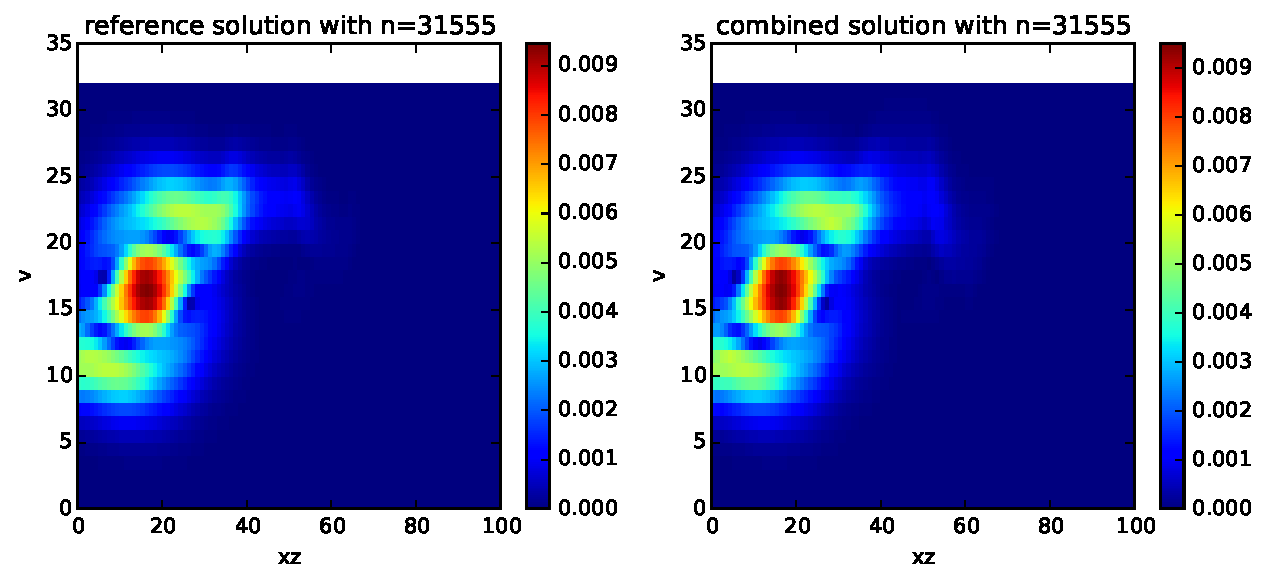
\includegraphics[width=\textwidth]{../fig/ref_and_combi}
	\caption{Reference solution and combined solution with $\vec n = (3,1,5,5,5)$ and $\lmin = (3,1,4,4,4)$.}
	\label{fig:ref_and_combi}
\end{figure}

\begin{figure}[h]
	\centering
	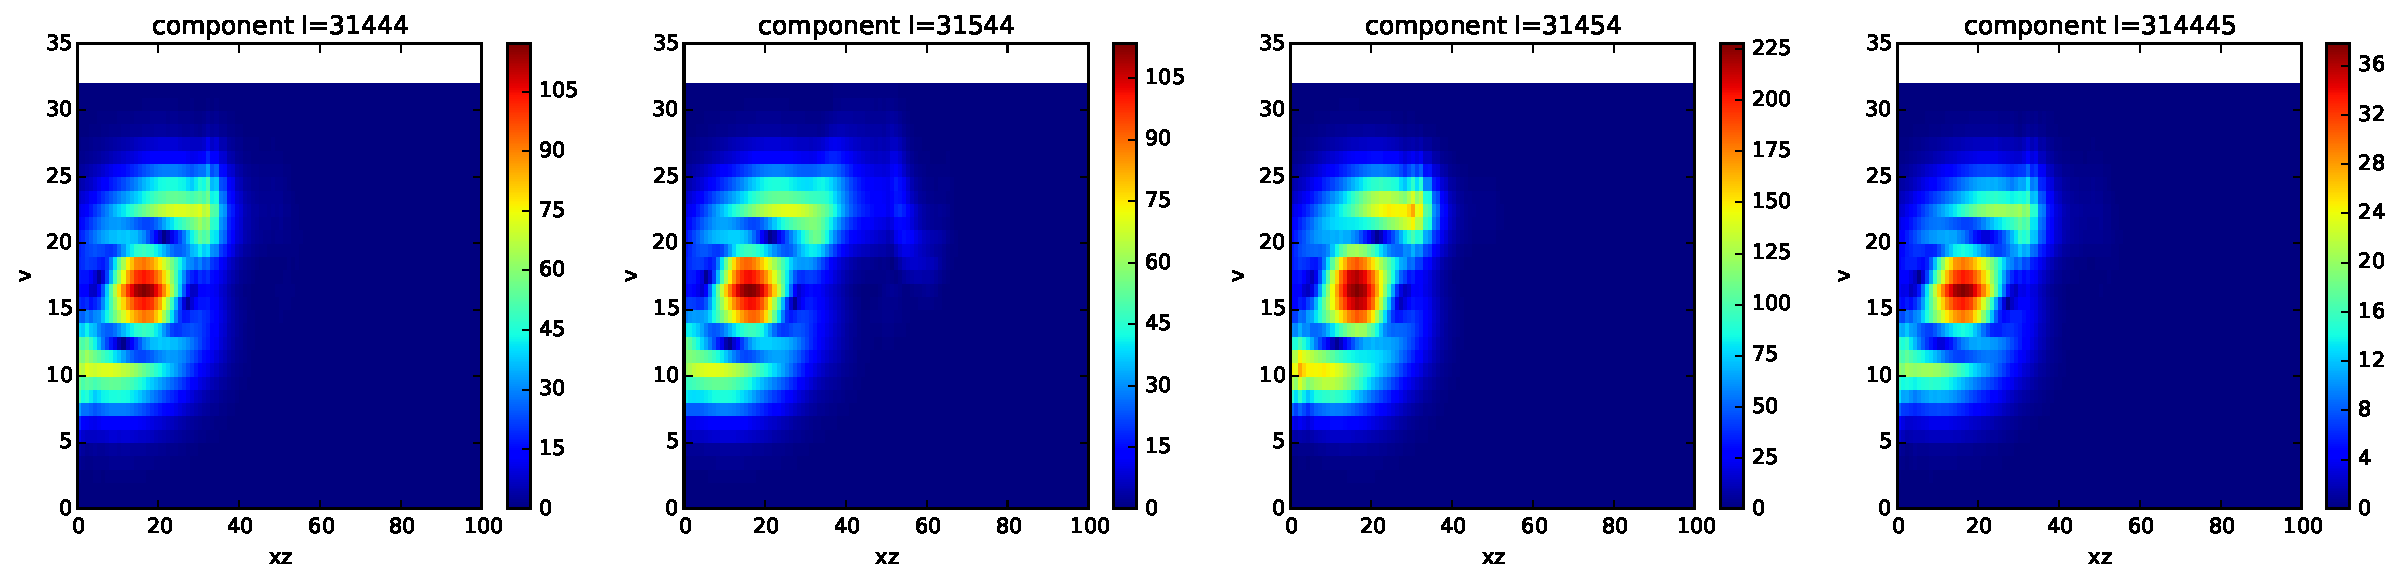
\includegraphics[width=\textwidth]{../fig/components}
	\caption{Individual component solutions corresponding to the combination technique with $\vec n = (3,1,5,5,5)$ and $\lmin = (3,1,4,4,4)$.}
	\label{fig:components}
\end{figure}

\begin{itemize}
	\item Figure~\ref{fig:ref_and_combi} shows a two-dimensional slice of the absolute value of $g$ (The $z$ and $x$ direction are merged together). The slice was taken at $\mu = 0.125$ (in unit hypercube coordinates). 
	\item The magnitude of the reference solution and combined solution in Figure~\ref{fig:ref_and_combi} are normalized.
	\item The combined solution was computed combining after each time step.
	\item The component solutions in Figure~\ref{fig:components} were computed in an individual simulation run (they are not the final results of the combination technique that was used in Figure~\ref{fig:ref_and_combi}).
	They would correspond to a combination technique where the component grids are only combined once in the end.
	They are not normalized to demonstrate the different magnitudes.
	\item The combined solution is more similar to the reference solution than any of the individual component solutions.
\end{itemize}

\subsection*{Computation of particle density moments and energies}

\begin{itemize}
	\item Figures~\ref{fig:q1} to~\ref{fig:q6} shows the different combination techniques applied to the quantities $q_i$ described in~\ref{sec:method_nrg}. 
	\item The error is expressed as $e_{q_i} = | q_i - q_{\text{ref},i} |$
	\item The results are similar as for the eigenvector and eigenvalue. The combined solution converges towards the reference solution and in most cases the combined solution is better than each of the individual component solutions. 
	\item Only in the case of $q_2$ there are some outliers. However, the reason for this needs further investigation.
\end{itemize}

\begin{figure}[h]
    \begin{subfigure}{0.5\textwidth}
        \includegraphics[width=\textwidth]{../fig/err_qoi_ref31888_1}
    \end{subfigure}%
    \begin{subfigure}{0.5\textwidth}
        \includegraphics[width=\textwidth]{../fig/err_qoi_lmax_1}
    \end{subfigure}%
    \caption{\textbf{(left)} Error of $q_1$ compared to the full grid solution with $\vec{l} = (3,1,8,8,8)$. resources for the different experiments. \textbf{(right)} Error of $q_1$ compared to the full grid solution with the corresponding target level $\vec{n}$. }
    \label{fig:q1}
\end{figure}

\begin{figure}[h]
    \begin{subfigure}{0.5\textwidth}
        \includegraphics[width=\textwidth]{../fig/err_qoi_ref31888_2}
    \end{subfigure}%
    \begin{subfigure}{0.5\textwidth}
        \includegraphics[width=\textwidth]{../fig/err_qoi_lmax_2}
    \end{subfigure}%
    \caption{\textbf{(left)} Error of $q_2$ compared to the full grid solution with $\vec{l} = (3,1,8,8,8)$. \textbf{(right)} Error of $q_2$ compared to the full grid solution with the corresponding target level $\vec{n}$. }
    \label{fig:q2}
\end{figure}

\begin{figure}[h]
    \begin{subfigure}{0.5\textwidth}
        \includegraphics[width=\textwidth]{../fig/err_qoi_ref31888_3}
    \end{subfigure}%
    \begin{subfigure}{0.5\textwidth}
        \includegraphics[width=\textwidth]{../fig/err_qoi_lmax_3}
    \end{subfigure}%
    \caption{\textbf{(left)} Error of $q_3$ compared to the full grid solution with $\vec{l} = (3,1,8,8,8)$. \textbf{(right)} Error of $q_3$ compared to the full grid solution with the corresponding target level $\vec{n}$. }
    \label{fig:q3}
\end{figure}

\begin{figure}[h]
    \begin{subfigure}{0.5\textwidth}
        \includegraphics[width=\textwidth]{../fig/err_qoi_ref31888_6}
    \end{subfigure}%
    \begin{subfigure}{0.5\textwidth}
        \includegraphics[width=\textwidth]{../fig/err_qoi_lmax_6}
    \end{subfigure}%
    \caption{\textbf{(left)} Error of $q_6$ compared to the full grid solution with $\vec{l} = (3,1,8,8,8)$. \textbf{(right)} Error of $q_6$ compared to the full grid solution with the corresponding target level $\vec{n}$. }
    \label{fig:q6}
\end{figure}



\clearpage
\appendix
\section{GENE parameter file used in the experiments}
\verbatiminput{parameter_example}


\end{document}

